%\documentclass[10pt,dvipsnames,slidestop,table]{beamer}
\documentclass[slidestop,compress,serif,10pt, handout]{beamer}
\mode<presentation>
\usepackage[accumulated]{beamerseminar}
\usepackage{beamertexpower}
%\usepackage{beamerthemeshadow}
\usepackage{pdfpages}
\usepackage{animate}
\usepackage{varwidth, tikz, pgfgantt}
\usepackage[latin1]{inputenc}
\usepackage[T1]{fontenc}
\usepackage{graphicx}
\usepackage{pdfpages}
\usepackage{amsmath, amssymb, amsthm}
\usepackage{amsfonts}
\usepackage{xspace, array}
\usepackage{color, xcolor, bm}
\usepackage{fancybox}
\usepackage{caption}
\captionsetup[table]{position=top}
\setbeamertemplate{footline}[frame number]

\usepackage{hyperref}

\usepackage{natbib}
\bibpunct{(}{)}{;}{a}{}{,}
\setbeamertemplate{navigation symbols}{}
%\usecolortheme{seagull}
%\useoutertheme{infolines}
\usefonttheme{structuresmallcapsserif}
%\usefonttheme[onlymath]{serif}
%\usetheme{Singapore}
%\usecolortheme{beaver}
%\usetheme{Goettingen}
\usecolortheme{dolphin}


\title[]{Modelling and challenges under a spatial epidemiology paradigm}
\author[Marta Blangiardo]{Marta Blangiardo}
\institute[]{Imperial College London \\ MRC-PHE Centre for Environment and Heath\\
\scriptsize m.blangiardo@imperial.ac.uk\\
\vspace{12pt}
%\footnotesize \emph{Joint work with}: \\
%Monica Pirani, Lauren Kanapka, Gary Fuller, Nicky Best, Silvia Liverani, Richard Atkinson
}
\date[]{LSHTM, XXX October 2017}
%\logo{
\includegraphics[height=0.85cm, width=3.3cm]{LogoNew.jpg}\hspace{133pt}}
%\titlegraphic{
\includegraphics[height=0.85cm, width=3.3cm]{LogoNew.jpg}\hspace{133pt}}
\begin{document}
\begin{frame}
\maketitle
\begin{center}
%\footnotesize
%\emph{Joint work with}: \\
%\underline{Gary Fuller}, Nicky Best, Marta Blangiardo, Silvia Liverani, Richard Atkinson\\
\begin{figure}

\includegraphics[height=0.87cm, width=3.4cm]{LogoNew.jpg}
\end{figure}
\end{center}
\end{frame}

%%%%%%%%%%%%%%%%%%%%%%%%%%%%%%%%%%%%%%%%%%%%%%%%%%%%%%%%%%%%%%%%%
%%%%%%%%%%%%%%%%%%%%%%%%%%%%%%%%%%%%%%%%%%%%%%%%%%%%%%%%%%%%%%%%%
\section{Me}
\begin{frame}\frametitle{}
\begin{description}
\item[Who I am] 
Senior Lecturer in Biostatistics\\
Imperial College,
Department of Epidemiology and Biostatistics\\
MRC-PHE Centre for Environment and Health\\
\vspace{4pt}\begin{center}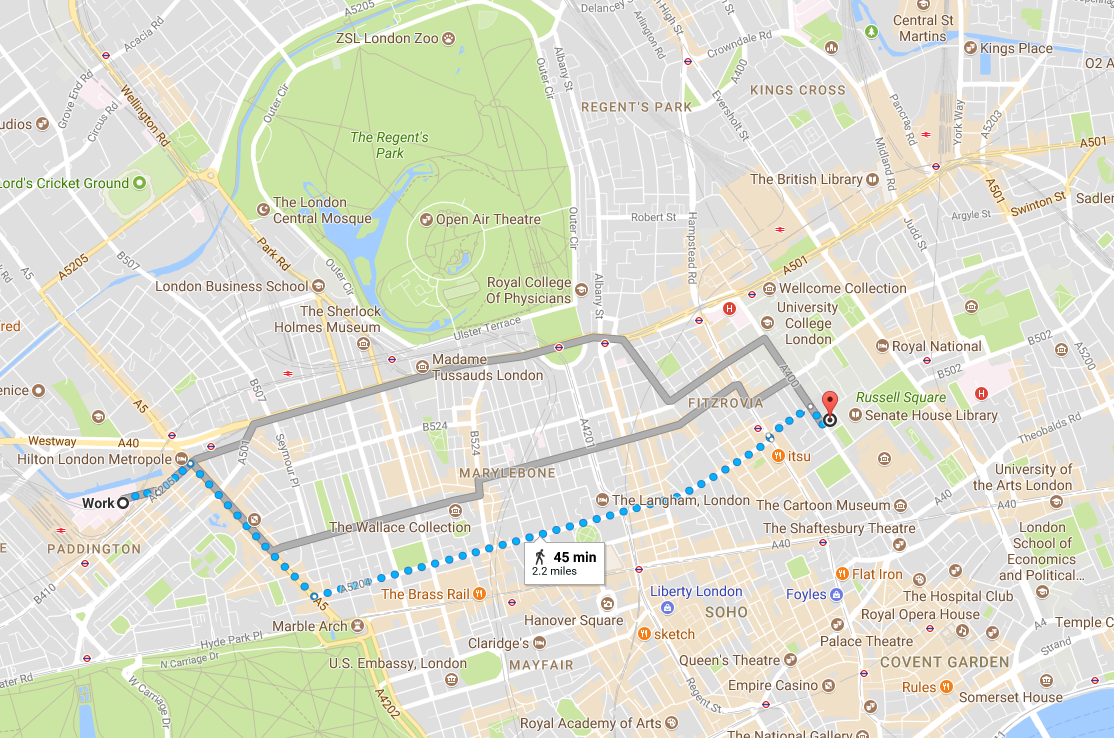
\includegraphics[width=4cm]{WorkMap.png}\end{center}
\item[What I do] Focus of my research is on the development of statistical methods to answer applied epidemiological questions

%\item[My talk] I will present my work on \bf{spatial epidemiology}\\
%\begin{itemize}
%\item Two main areas: \\
%$\Rightarrow$ epidemiological surveillance\\
%$\Rightarrow$ risk assessment
%\end{itemize}
\end{description}  \end{frame}
%%%%%%%%%%%%%%%%%%%%%%%%%%%%%%%%%%%%%%%%%%%%%%%%%%%%%%%%%%%%%%%%%
\begin{frame}\frametitle{My work on Environmental Epidemiology}
\begin{center}
\scalebox{.85}{\begin{tikzpicture}
%\draw[rounded corners=15pt,thick] (-16.8,-1.6) rectangle ++ (7.1,6.2);
\draw(-17,-4) node[align=center,font=\sffamily\fontsize{7}{7}\selectfont](Exp){\\ Environmental exposure\\ e.g. air pollution\\ noise, pesticides};
\node[below=0.1 of Exp, align=center,font=\sffamily\fontsize{7}{7}\selectfont](Mes){Measurements};
\node[below=0.1 of Mes, align=center,font=\sffamily\fontsize{7}{7}\selectfont](Mod){Modelled};
\node[above=0.5 of Exp, text=blue,align=center,font=\sffamily\fontsize{7}{7}\selectfont](Methods1){Space-time regression};
\node[below=0.5 of Mod, text=red,align=center,font=\sffamily\fontsize{7}{7}\selectfont](Chall1){Misalignment\\ Measurement error\\ Correlated data\\ Computational (big data)};
\node[right=4 of Exp, align=center,font=\sffamily\fontsize{7}{7}\selectfont](Health){Health data\\ (EHR)\\};
\node[below=0.18 of Health, align=center,font=\sffamily\fontsize{7}{7}\selectfont](HES){Hospital Admissions};
\node[below=0.1 of HES, align=center,font=\sffamily\fontsize{7}{7}\selectfont](Mort){Mortality Registry};
\node[above=0.5 of Health, text=blue,align=center,font=\sffamily\fontsize{7}{7}\selectfont](Methods2){Clustering;\\ Surveillance};
\node[below=0.5 of Mort, text=red,align=center,font=\sffamily\fontsize{7}{7}\selectfont](Chall2){Correlated conditions;\\ Space-time resolution};
\draw [->, thick] (Exp.east) to (Health.west);
\node[below right = 0.2 of Exp, align=center,font=\sffamily\fontsize{7}{7}\selectfont, text=red](Chall3){Correlation;\\ Residual confounding\\ Dose-response};
\node[above=1.1 of Chall3, text=blue,align=center,font=\sffamily\fontsize{7}{7}\selectfont](RA){Risk assessment};

\node[below=4.2 of RA, align=center,font=\sffamily\fontsize{7}{7}\selectfont, text=red](Overarching){Uncertainty propagation \& feedback;  Missing data};


\end{tikzpicture}}
\end{center}

In this talk\\
\begin{itemize}
\item Two main areas: \\
$\Rightarrow$ epidemiological surveillance\\
$\Rightarrow$ risk assessment
\end{itemize}
\end{frame}
\end{document}
